\documentclass[aip,cp,amsmath,amssymb,reprint]{revtex4-2}

\usepackage{graphicx}
\usepackage{dcolumn}
\usepackage{bm}

\usepackage[utf8]{inputenc}
\usepackage[T1]{fontenc}
\usepackage{mathptmx} 

\begin{document}
\title{The Title Goes Here with Each Initial Letter Capitalized}% Force line breaks with \\
\author{Brian L. Frost} % Write as First name Surname
 \email[Corresponding author: ]{b.frost@columbia.edu}
\affiliation{
Department of Electrical Engineering, Columbia University, 500 W. 120th St., Mudd 1310, New York, New York 10027, USA
}
\author{C. Elliott Strimbu}%
 \email{ces2243@cumc.columbia.edu}
\affiliation{
Department of Otolaryngology Head and Neck Surgery, Vagelos College of Physicians and Surgeons, Columbia University, 630 W. 168th St., New York, New York 10032, USA
}

\author{Elizabeth S. Olson}
 \email{eao2004@cumc.columbia.edu}
\affiliation{
Department of Otolaryngology Head and Neck Surgery, Vagelos College of Physicians and Surgeons, Columbia University, 630 W. 168th St., New York, New York 10032, USA
}
\affiliation{
Department of Biomedical Engineering, Columbia University, 351 Engineering Terrace, 1210 Amsterdam Ave., New York, New York 10027, USA
}


\begin{abstract}
	Intra-organ of Corti displacement measurements made via optical coherence tomography have provided significant information about cochlear micromechanics in recent years. However, several ambiguities inherent to this modality have complicated interpretation of these measurements, along with causing apparent disagreements between data from different groups. Among these ambiguities is the fact that optical coherence tomography measures only a one-dimensional projection of a three-dimensional motion onto an axis with no physiological relevance. Moreover, the optical axis may make a significant angle with the basilar membrane normal, meaning that structures measured in a single measurement may lie in different tonotopic cross-sections. We have developed a method which accounts for both of these ambiguities inherent to optical coherence tomography measurements to reconstruct the two-dimensional longitudinal-transverse components of displacements of structures within the organ of Corti. This is performed via taking data at multiple longitudinal positions at two viewing angles without any \textit{a priori} knowledge of the measurement locations or viewing angles. We present a sample data set in which we have applied this program to reconstruct the transverse-longitudinal motion of the base of the outer hair cells in the base of the sensitive gerbil cochlea, which suggest that certain disparate phase response measurements between multiple groups may be explained by taking the measurement angle into account.
\end{abstract}

\maketitle

\section{\label{sec:intro}Introduction}
\par{Historically, the in vivo study of cochlear mechanics has been limited to measurements of the basilar membrane (BM). The advent of optical coherence tomography (OCT) in the last decade has allowed for vibrometry at a depth, facilitating the study of intra-organ of Corti complex (OCC) motions. Of particular interest is the motion of the electromotile outer hair cells (OHCs), which play an important role in the amplifying vibration responses and increasing the range of sound-pressure levels (SPLs) over which hearing operates.}
\par{Several groups have presented OCT measurements of OHC motion in the base of the sensitive gerbil cochlea. In some instances, these measurements have differed significantly from one another. In particular, groups have reported disparate phase differences between displacements in the ``OHC region" and at the BM.}
\par{Several aspects complicate these measurements. The first is that the term ``OHC region" is ill-defined; the OHCs are 40 $\mu$m long and 10 $\mu$m wide, and come in rows of three per longitudinal cross-section. Mechanical intuition may lead one to believe that the apical surface of the OHCs, called the reticular lamina (RL), may move differently from the basal surface attached to the Deiters' cells as the OHC compresses and expands due to electromotility. Generally, it is naive to assume that the entire ~120 $\mu$m$^2$ OHC region moves uniformly.}
\par{A second complication is that measurements are taken at an angle with respect to the orientation of the cochlea, unknown \textit{a priori}. This means that (1) displacements measured via OCT are projections of the three-dimensional motion onto an unknown axis, and (2) measured points at the OHC and BM within a single measurement may lie in different longitudinal cross-sections.}
\par{The first of these ambiguities is discussed by Cooper et al, wherein the authors discuss the hypothetical scenario that OHCs exhibit some fluid-like elliptical motions\cite{cooper2018}. Their model showed that the phase difference between measured OHC and BM motion relied heavily on the viewing angle, with any deviation between -180 and +180 degrees being achievable. The viewing angle is critical for the assessment of phase differences between OHC and BM motion.}
\par{The second of these ambiguities is discussed by Frost et al, wherein we developed a program which measured the relative anatomical displacements between structures measured via OCT\cite{frost2022}. We used this program to account for the longitudinal displacement between measured OHC and BM, and showed that this correction significantly affected the character of OHC phase re BM. This included a discrepancy of up to 90 degrees between displacement-accounted and single-measurement phases at high frequencies.}
\par{With these complications in mind, it is difficult to interpret presented OCT measurements of OHC displacement reported without a viewing angle. The group of Ren has achieved RL and OHC displacement measurements (via an interferometer similar to OCT) taken at a purely transverse angle, both in gerbil and mouse\cite{he2018,ren2016}. They show that RL phase leads BM at low frequencies, but that this lead decreases monotonically and near-linearly until the structures are in phase at about 80\% of the best frequency (BF). After this zero crossing, the RL re BM phase continues its monotonic decrease, with the RL lagging the BM at near- and supra-BF frequencies.}
\par{Meanwhile the other hand, our displacement-accounted data (i.e. OHC and BM in the same tonotopic cross-section) taken at a viewing angle with a significant longitudinal component shows a phase difference of a very different character. We see that OHC leads BM across frequency, including at high frequencies -- where Ren et al see an 80 degree \textit{lag}, we see a 90 degree \textit{lead}.}
\par{We have developed a method to isolate the transverse and longitudinal components of motion of structures within the OCC, wherein we account both for the longitudinal displacement between structures and the projection incurred by the viewing angle. Similar to the work of Lee et al, we do so by taking measurements at multiple viewing angles\cite{lee2016}. Our method requires no \textit{a priori} knowledge of either measurement angle, or of the positions of the structures being measured. We employ a linear approximation of the longitudinal direction at acquisition time, followed by \textit{post hoc} registration of structures measured at several longitudinal locations and viewing angles. We then backproject the measured displacements to achieve a reconstructed longitudinal-transverse profile of a structure's motion.}
\par{We present the method, an analysis of its fidelity with respect to viewing angle, as well as \textit{in vivo} data from the base of the gerbil cochlea in which the longitudinal-transverse motion at the base of several OHCs has been reconstructed. In this sample data set, our reconstructed transverse displacements are consistent with previously measured pure-transverse displacements. We also see that longitudinal OHC displacement is generall smaller than transverse OHC displacement in magnitude, and ~180 degrees out of phase (with respect to our chose coordinate system) with transverse OHC displacements across frequency.}

\section{\label{sec:methods}Methods}

\subsection{\label{sec:acquisition}Acquisition}
\par{The acquisition process follows a few simple steps: (1) prior to acquisition, ensure the BM looks as horizontal as possible in the orienting B-Scan, (2) determine the approximate longitudinal direction and take measurements of a single structure at multiple longitudinal locations, (3) rotate the preparation and try to isolate similar cross-sections with the BM appearing horizontal in the orienting B-Scan, (4) again, find the approximate longitudinal direction and take measurements of the same structure at multiple longitudinal locations.}
\par{Orienting the preparation so that the BM appears horizontal in each cross-section ensures that the radial component of the optic axis is approximately zero. This is important, as we are attempting to simplify our problem to two dimensions – transverse and longitudinal. Failing to account for this radial angle will make our two-dimensional reconstruction impossible.}
\par{Determining the approximate longitudinal directions works via a linear approximation of the cochlea’s anatomical coordinates, similar to the planar approximation employed in Frost et al, 2022. As we only need the longitudinal direction for acquisition, this is a simpler process – we use ThorImage and locate a landmark in some cross-section; for example, we can choose the base of the OHC, or the thickest part of the BM. We record the optical coordinates at these positions, $p_1 = (x_1,y_1,z_1)$ and $p_2 = x_2, y_2, z_2)$. The difference between these points is a linear approximation of a vector in the longitudinal direction, so the unit longitudinal vector is
	\begin{equation}
		\label{eqn:lunit}
		l = \frac{p_2-p_1}{|p_2-p_1|}.
	\end{equation}
This process is illustrated in panels A and B of Fig. \ref{fig:acq}.}
\par{We can find points of measurement at fixed increments along the longitudinal direction. If we start at a point $q_0$, and want to measure $N$ points over longitudinal distance $L$, we measure at 
	\begin{equation}
		\label{eqn:points}
		q_n = q_0 + \frac{nL}{N}l,\;n=0,1,\ldots,N-1.
	\end{equation}
This is illustrated in panel C of Fig. \ref{fig:acq}.}
\par{We take volume scans after each run so that outside of the time pressure of an experiment, we can apply our more complex orientation program\cite{frost2022}. In doing so, we can assess the accuracy of our assumption that the radial component of our measurement axis is 0, as well as the direction of the longitudinal vector.}

\subsection{\label{sec:registration}Registration}

\par{As we have made sure to remove the radial component of motion from our measurements, we can assume the optical $z$ axis is comprised of only longitudinal ($l$) and transverse ($t$) components. We write the optical axis’ unit vector as a two-dimensional vector in anatomical
coordinates, $z = (z_l, z_t)$.
}
\par{Eqn. \ref{eqn:lunit} is used in the acquisition step to find the longitudinal vector $l$, which has optical $x$, $y$ and $z$ components. The $z$ component of this vector represents the amount of longitudinal motion that is projected onto the optical axis, $z_l$. To find the $t$ component of $z$, we need only to recall that $z$ is a unit vector, so that $z_l^2 + z_t^2 = 1$. Using the notation from Eqn. \ref{eqn:lunit}, we have

	\begin{align}
		z_l &= \frac{z_2-z_1}{|p_2-p_1|},\\
		z_t &= \sqrt{1-z_l^2}.
	\end{align}
This is illustrated in panel C of Fig. \ref{fig:acq}.}
\par{Knowing this, we can relate the OHC and BM longitudinal locations within a single measurement. If the structures along a single measurement axis are spaced $\Delta z$ apart, then the OHCs lie $\Delta l = z_l \Delta z$ apical of the BM. The measured BM $\Delta l$ apical of this measurement is thereby in the same longitudinal cross-section as the OHC in the first measurement. We call these BM and OHC measurements \textit{aligned} to one another. At each measurement angle, we compose a list of all aligned OHC and BM measurements. This process is illustrated in panels D and E of Fig. \ref{fig:acq}.}
\par{To register points to one another between viewing angles, we use the phase of BM motion. By matching the phase responses of BM measurements taken at different viewing angles, we can register the cross-sections in which these BM motions were measured. This operates under the assumption that BM motion is entirely transverse, so that its phase response at each cross-section will be the same at each viewing angle. }
\par{Having registered BM points to one another, we can then consult our list of aligned BM-OHC pairs. The OHCs aligned to registered BM positions are also registered, allowing us to isolate the same OHCs at different viewing angles.}

\begin{figure}[h]
	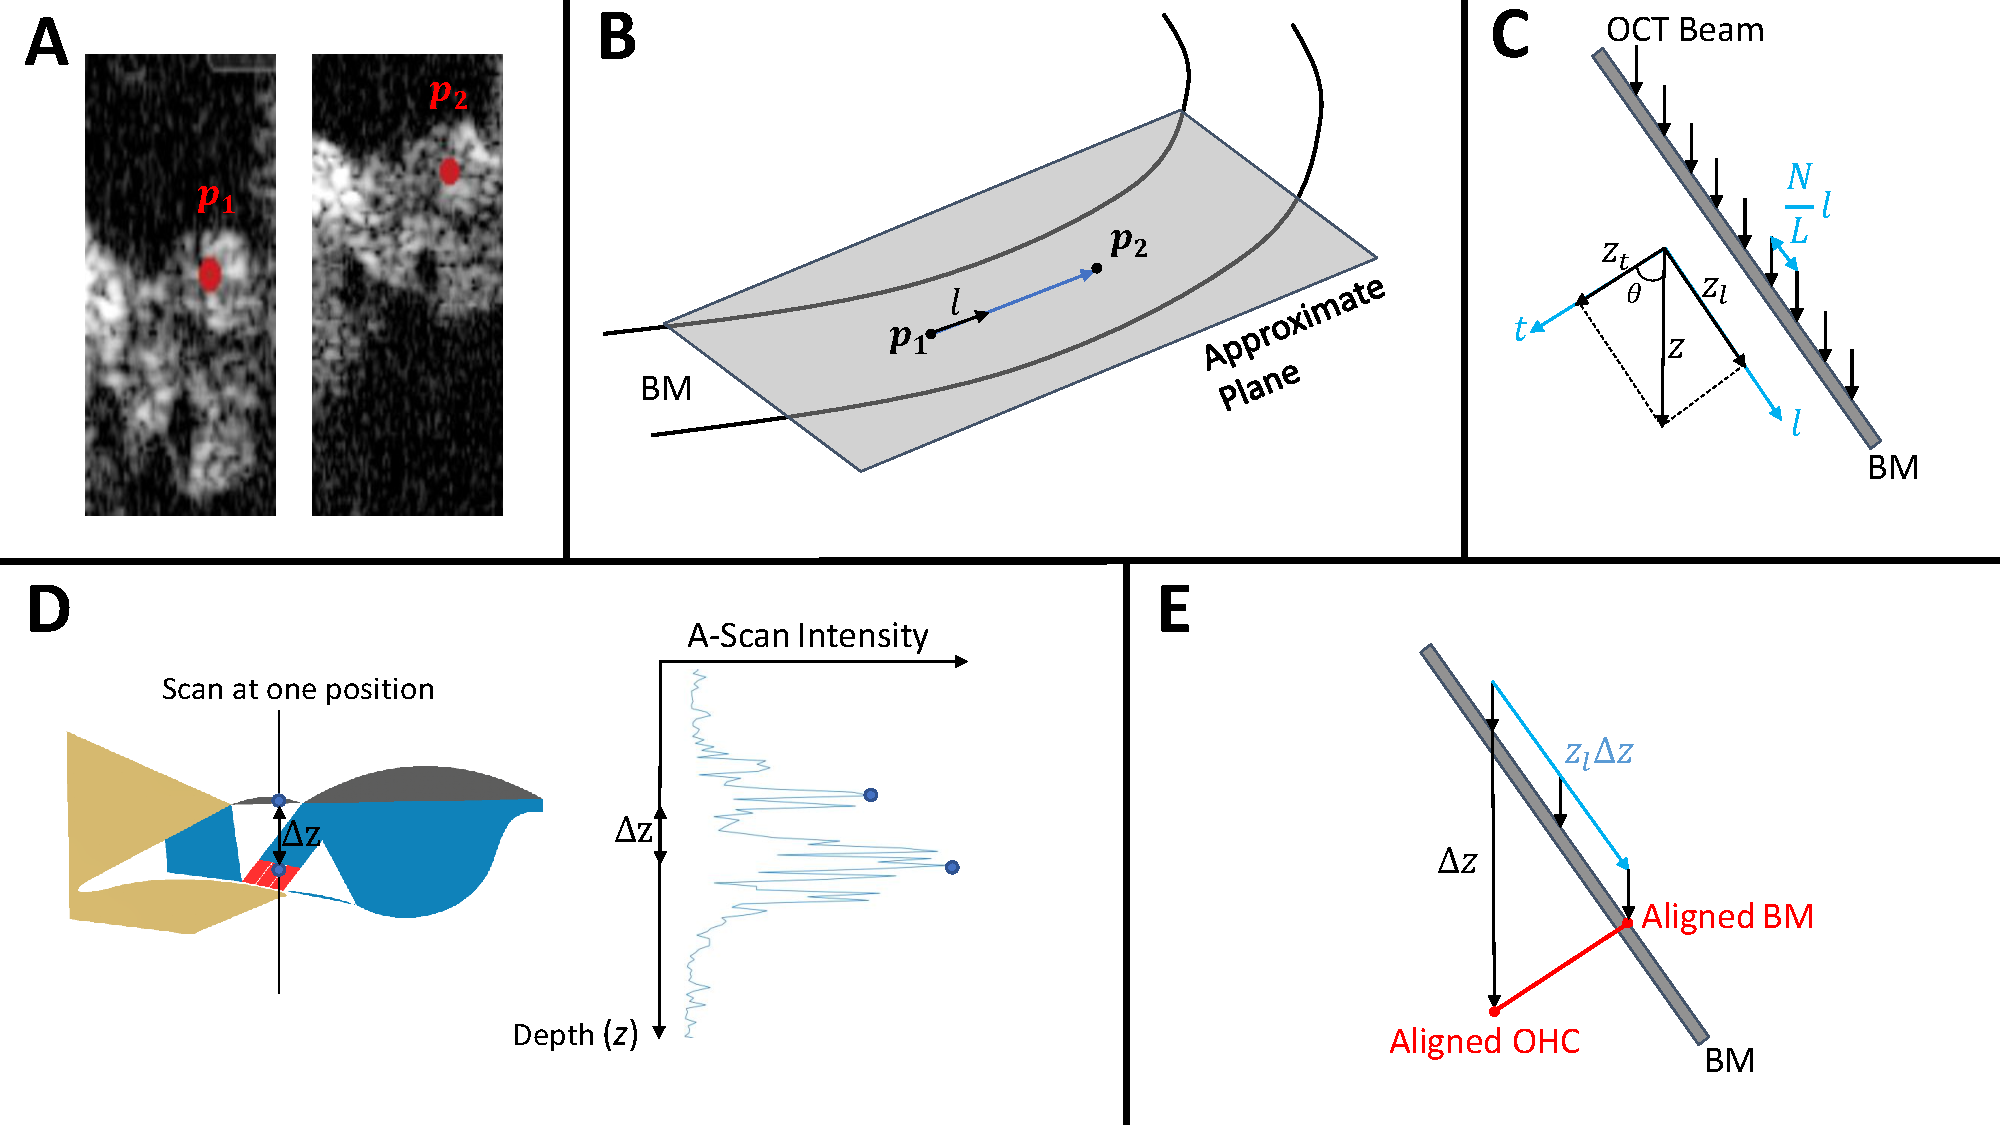
\includegraphics[width=\textwidth]{Figures/AlignmentExample.pdf}
	\caption{\textbf{A} -- Two parallel B-Scans from a single volume, about 50 $\mu$m apart, on which we have marked points $p_1$ and $p_2$ used to determine the longitudinal direction $l$. We have selected the landmark to be the BM at its widest point. We have ensured that the BM appears approximately horizontal in each B-Scan, so as to remove all radial displacement contributions. \textbf{B} -- A cartoon of the BM, with true longitudinal axis varying in space. We have approximated this axis by a line passing through both $p_1$ and $p_2$. \textbf{C} -- A cartoon of the BM projected onto the longitudinal-transverse plane, in which our A-Scans lie. We take A-Scans along the $z$ axis at multiple evenly spaced longitudinal positions. We can determine the anatomical components of the $z$ vector via geometry, knowing $l$ and knowing that $z$ has unit length. \textbf{D} -- A cartoon of the organ of Corti complex and an experimentally acquired A-Scan. We measure the distance between OHC base and BM in the A-Scan, $\Delta z$, to determine the longitudinal displacement between these structures. \textbf{E} -- A cartoon of the BM in the longitudinal-transverse plane similar to \textbf{C}. The OHC at a measurement position is $z_l \Delta z$ apical of the BM at that same position. This OHC's \textit{aligned} BM point is that which is measured at this same longitudinal position.}
	\label{fig:acq}
\end{figure}

\subsection{\label{sec:reconstruction}Reconstruction}
\par{Each OCT measurement is a projection of a true 3-D motion onto the optical $z$ axis. In the current context, we have made efforts to eliminate the representation of radial motion in our projection,so that the problem can be framed as the projection of a 2-D longitudinal-transverse \textit{true motion} $d$ onto a 2-D transverse-longitudinal $z$ axis, forming the \textit{projected motion} $\delta$.}
\par{Above we describe the method by which we determine the $z_l$ and $z_t$ components of the optical axis in each experiment. The projection onto this axis is given by the dot product
     \begin{equation}
         \delta = z \cdot d = \begin{pmatrix}z_l& z_t\end{pmatrix}\begin{pmatrix}d_l\\d_t\end{pmatrix}.
     \end{equation}
}
\par{At each angle, if we are truly measuring at one position, $d$ will remain the same and $z$ will     change. If we take measurements at two angles, we form the system of equations:
     \begin{equation}\label{projmat}
         \begin{pmatrix}\delta_1 \\ \delta_2\end{pmatrix} = \begin{pmatrix}l_1 & t_1\\l_2 & t_2\end{pmatrix}\begin{pmatrix}d_l\\d_t\end{pmatrix},
     \end{equation}
     where the rows of the matrix are the $z$ axes corresponding to each angle, and $\delta_i$ is the     projection measured at the $i^\text{th}$ angle.
}
\par{We measure $\delta_i$ and determine the $l$ and $t$ components of the $z$ axis as described above. We want to reconstruct $d$, which can be done simply by inverting the matrix in Equation \ref{projmat}. This is possible if and only if the rows of the matrix are linearly independent, i.e. if the measurement axes are not colinear. So long as we measure at two sufficiently distinct (to be quantified shortly) angles, we can reconstruct $d$ by performing the matrix inverse:
     \begin{equation}\label{fullreconstruct}
         \begin{pmatrix}d_l\\d_t\end{pmatrix}=\frac{1}{l_1 t_2 - l_2 t_1}\begin{pmatrix}t_2&-t_1\\-l_2  & l_1\end{pmatrix}\begin{pmatrix}\delta_1\\ \delta_2\end{pmatrix}.
     \end{equation}
}
\par{Achieving measurements of the same structures at different angles is constrained by the preparation. In practice, a 15 degree rotation is tractable in our preparation, but significantly larger angles are not consistently achievable. Of course, one could attempt to reconstruct from measurements taken at angles with only a fraction of a degree of discrepancy, but intuitively this will be unreliable due to the precision of our devices and the noise in the displacement signal.}
\par{The precision of our reconstruction can be found via the \textit{condition number} $\kappa$ of our projection matrix in Eqn. \ref{projmat}. The condition number is defined as
     \begin{equation}
         \kappa (A) = \frac{|\sigma_{max}|}{|\sigma_{min}|},
     \end{equation}
where $\sigma_{max}$ and $\sigma_{min}$ are the maximum and minimum singular values of matrix $A$. The condition number of a matrix represents how ``well-posed" a system of equations is, i.e. how close to singular the matrix is. A matrix with a large condition number will amplify noise significantly more than a matrix with a small condition number. The ``rule of thumb" is that noise is multiplied by around $\kappa$. That is, for $\kappa \approx 10^k$, about $k$ digits of precision are lost via the matrix multiplication. Note that a matrix and its inverse have the same condition number.
}
\par{Table \ref{kappas} shows condition numbers for some possible angular deviations. Condition number does not depend on the absolute angle, but only the absolute difference between the two measurement angles. We should note that our usual precision is on the order of $0.1$ nm, and our signal at higher dB SPL is in the range of 1-10 nm.}
 
\begin{table} 
\begin{center}
    \begin{tabular}{|c|c|}
        \hline
        Angular deviation & Condition number $\kappa$ \\
        \hline
        20$^\text{o}$ & 5.67\\
        15$^\text{o}$ & 7.60\\
        10$^\text{o}$ & 11.43\\
        5$^\text{o}$ & 22.90 \\
        1$^\text{o}$ & 114.59\\
        \hline
    \end{tabular}
    \caption{A table of condition numbers for the projection matrix at possible measurement angular deviations.}
\label{kappas}
\end{center}
\end{table}
 
\par{These should be more-or-less known and kept in mind when analyzing data reconstructed via this method. The realized 15-degree angle will lead to an eight-fold increase in the noise level, which means our results are accurate to about 0.8 nm.}


\section{\label{sec:results}Results}

\par{We have employed the method described above in the base of the gerbil cochlea, with measurements taken through the round window membrane at angles of approximately 45$^\text{o}$ and $60^\text{o}$. We take data at 11 positions spaced 15 $\mu$m apart longitudinally at each angle, ensuring that at each point we measure a position at the base of the OHCs. We stimulate with one-second, 15-frequency multitone stimuli at 80 dB SPL.}
\par{As we step longitudinally along the cochlea, we expect to see the phase response at the BM to vary along with the tonotopic cross-section. This behavior is displayed in Fig. \ref{fig:acrossl}, providing evidence that our acquisition method is truly stepping along the tonotopic axis.}

\begin{figure}[h]
	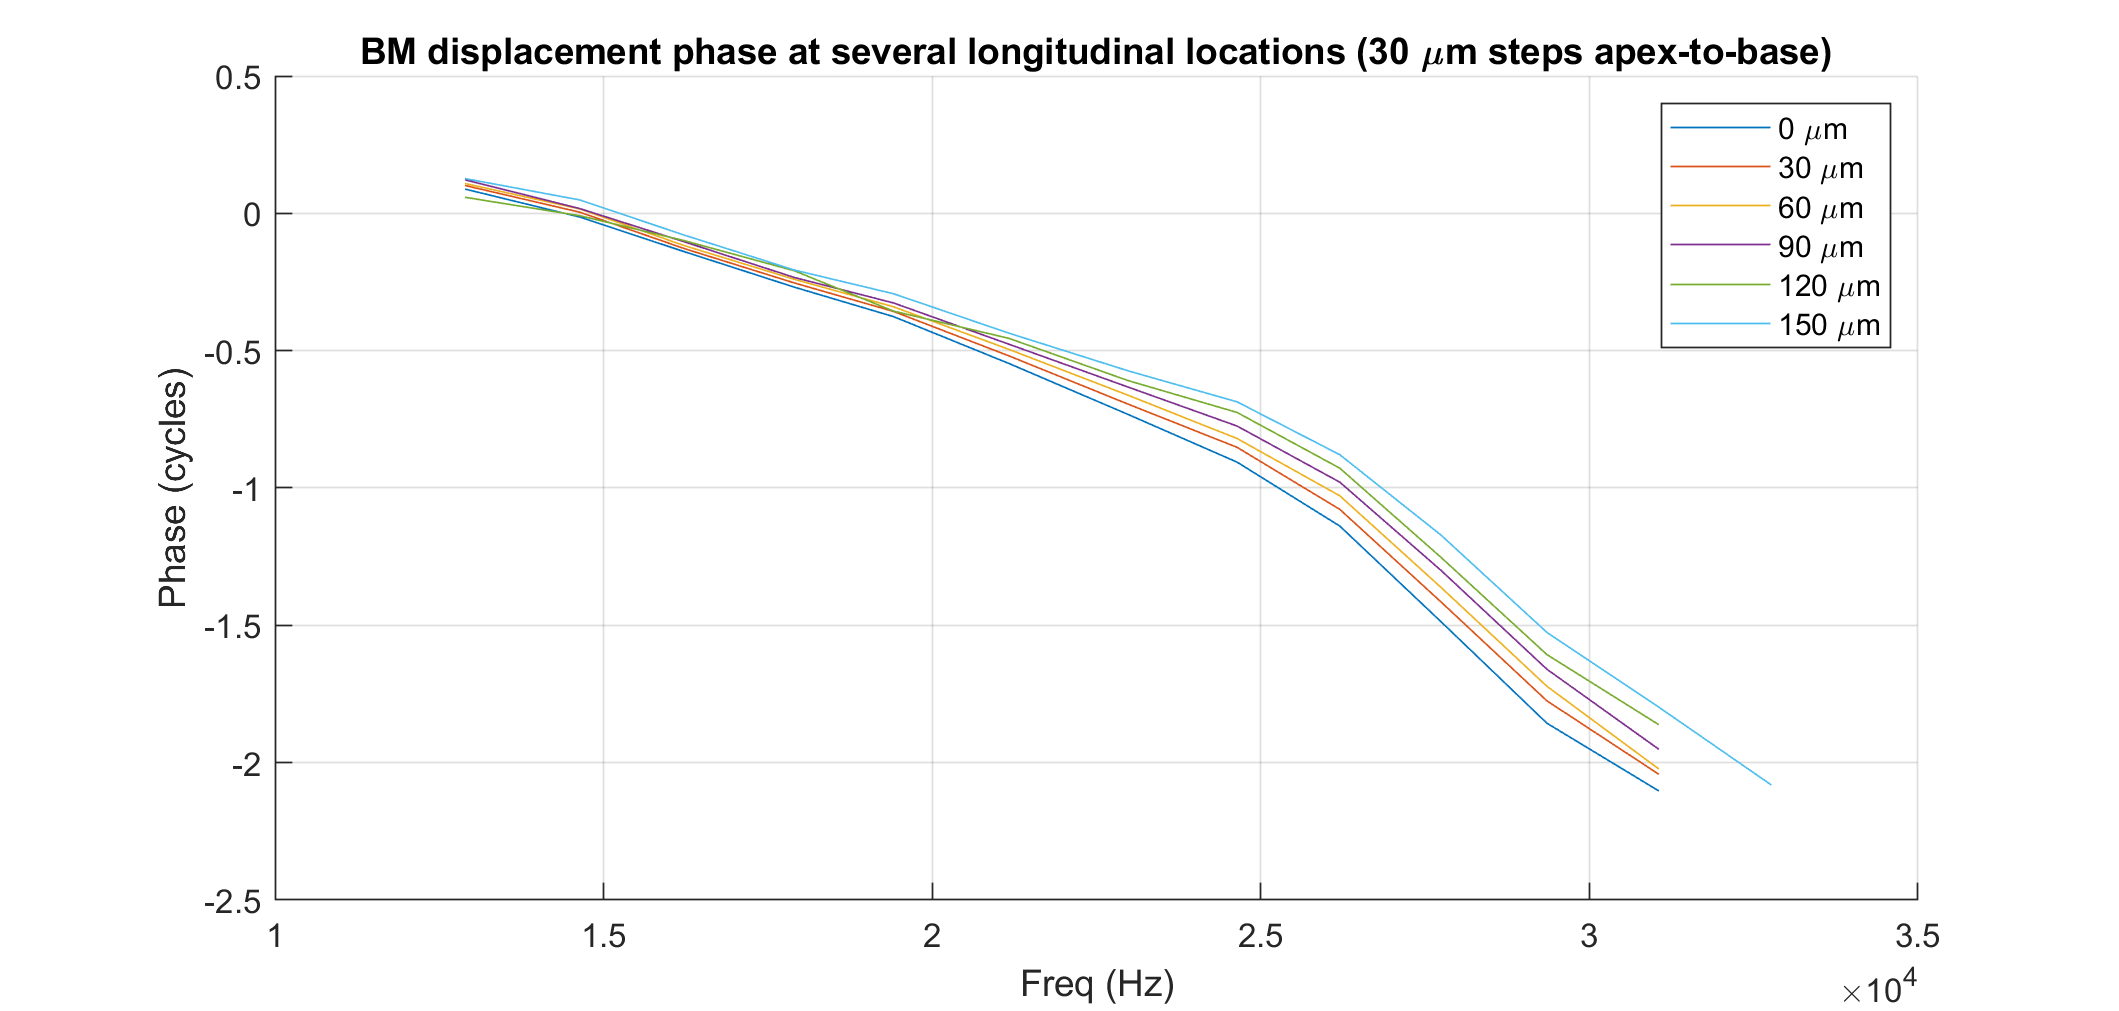
\includegraphics[width=.7\textwidth]{Figures/displacementacrossl_MOH.png}
	\caption{Phase of BM displacement measured in response to 80 dB SPL 15-frequency multitone stimulus, taken at several points along the longitudinal axis of the cochlea. The OCT beam is oriented at $45^\text{o}$ to the BM, and we have stepped 15 $\mu$m at a time along the cochlea over a 150 $\mu$m range. We display every other step here to make clear the travelling wave pattern of the displacement as we step from apex to base.}
	\label{fig:acrossl}
\end{figure}

\par{As for the registration process, Fig. \ref{fig:matching} shows matched BM phases taken at two different angles. While we did not know the overlap of the measured regions at each angle \textit{a priori}, we have found this 60 $\mu$m region of longitudinal overlap \textit{post hoc}. As each of these positions is one longitudinal measurement step apart  at their respective angles, this provides evidence that we have correctly taken uniform longitudinal steps at both angles.}
\begin{figure}[h]
	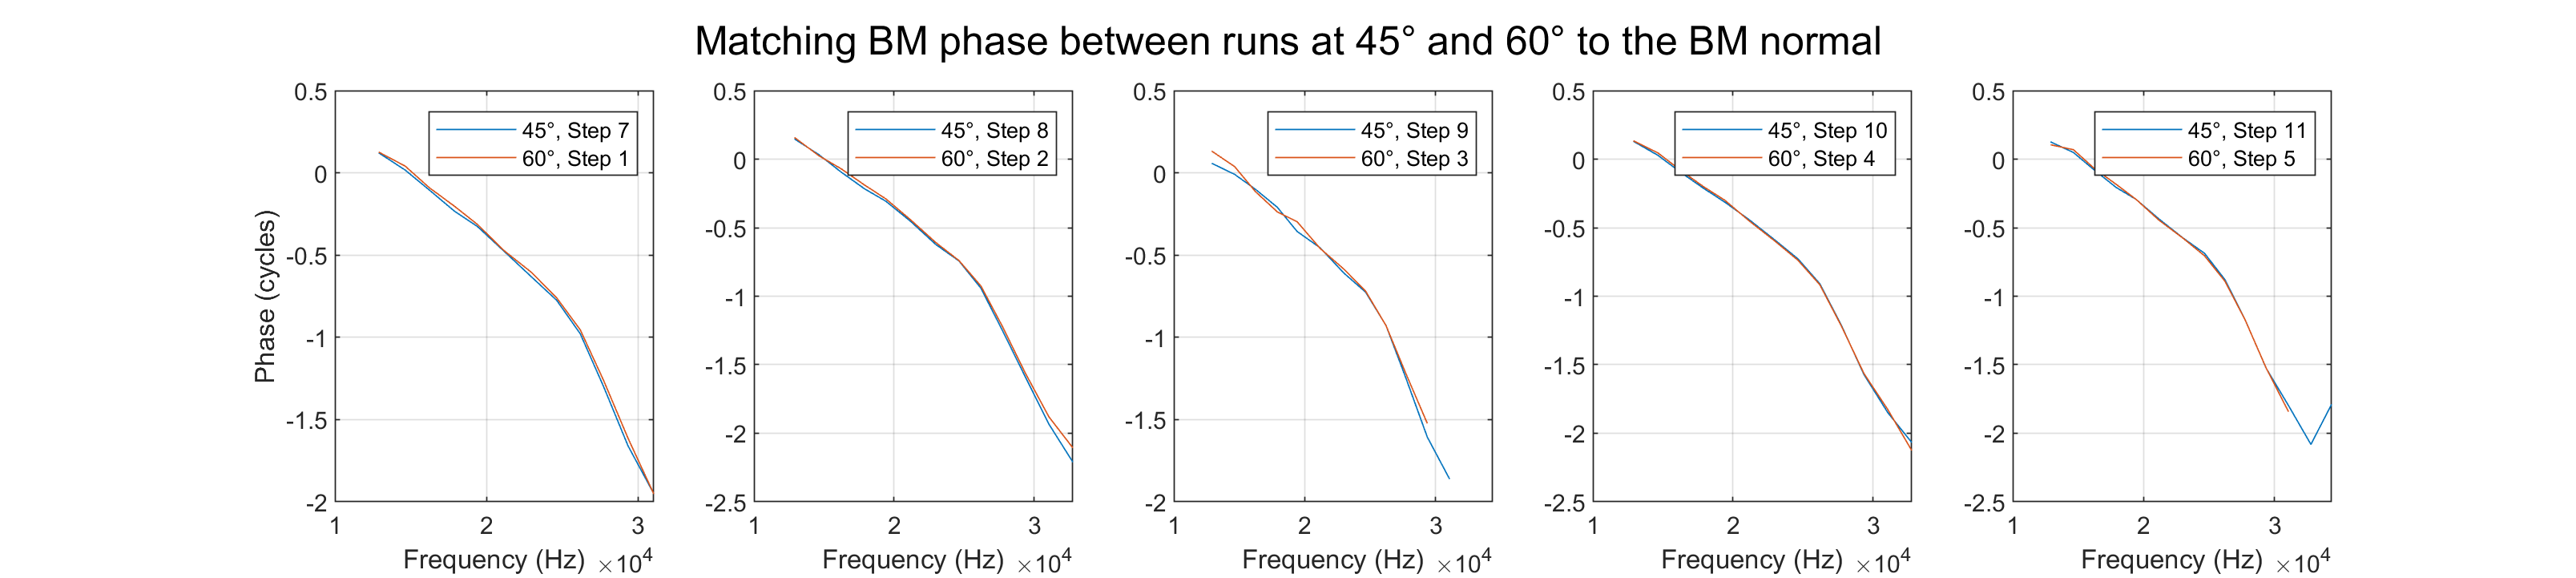
\includegraphics[width=\textwidth]{Figures/matching_MOH.png}
	\caption{Five matched BM phase plots used for registering locations between measurement angles. In each subplot, we show BM displacement phase measured at two different angles with maximum overlap. Each ``step" from left-to-right is measured 15 $\mu$m basal of the previous step.}
	\label{fig:matching}
\end{figure}
\par{Applying our reconstruction method to the associated aligned OHCs we arrive at the two-dimensional frequency responses presented in Fig. \ref{fig:ohcresp}. At all registered OHC base locations, we see that transverse OHC motion is significantly larger than longitudinal OHC motion across the bulk of the frequency range at 80 dB. Reconstructed transverse OHC displacement phase undergoes the linear lead-to-lag transition measured by Renet al and He et al, with zero-crossing near 0.8BF\cite{he2018,ren2016}.}
\begin{figure}[h]
	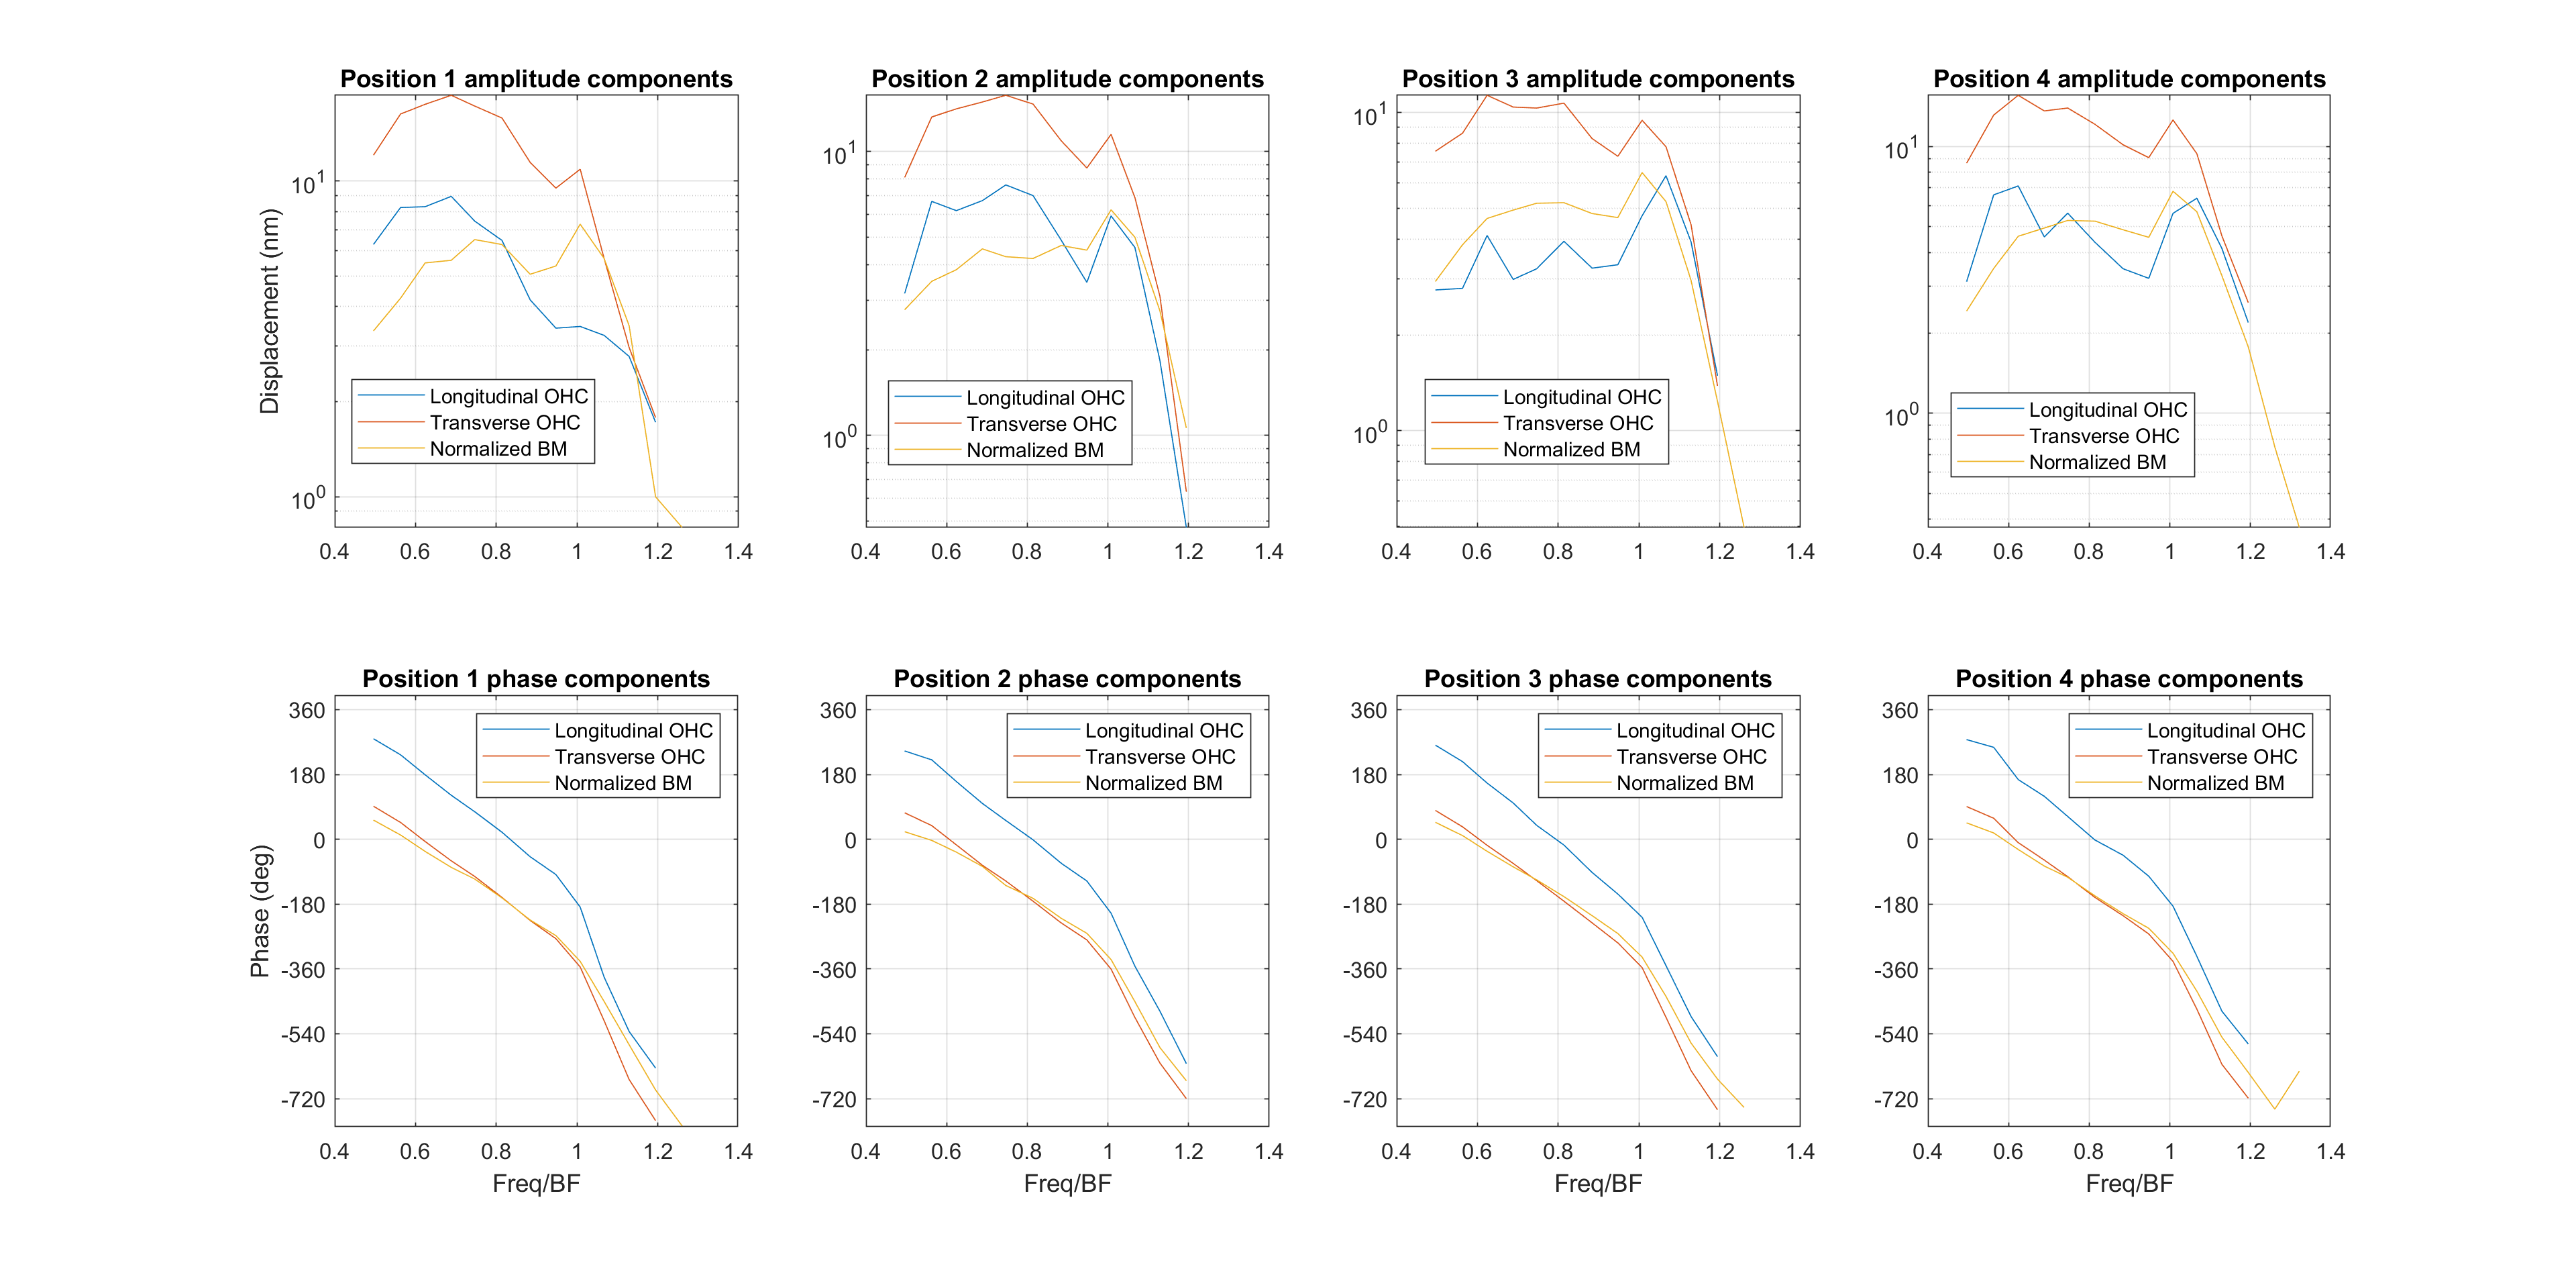
\includegraphics[width=\textwidth]{Figures/ampphase_MOH.png}
	\caption{Amplitude and phase response of transverse and longitudinal OHC motion, reconstructed at 4 different longitudinal positions spaced 15 $\mu$m apart. Presented also is the BM displacement at this position, taken from the aligned BM displacement with 45$^\text{o}$ measurement angle. We have normalized this BM displacement value by multiplying by $\sqrt{2}$ -- the theoretical geometric loss incurred by measuring a purely transverse BM motion at a 45$^\text{o}$ angle.}
	\label{fig:ohcresp}
\end{figure}
\par{Interestingly, the longitudinal displacement phase leads transverse displacement phase by about 180 degrees. With respect to our coordinate system, this means that towards-BM transverse displacement is in phase with basal-to-apical longitudinal displacement, with their 2-D transverse-longitudinal displacements being shaped approximately linearly.}

\section{\label{sec:conclusion}Conclusion}

\par{We have developed and presented the application of a method via which longitudinal-transverse 2-D intra-OCC displacements can be reconstructed from 1-D OCT measurements, without any \textit{a priori} knowledge of the measurement angles or measurement locations. We have presented the application of this method to reconstructing the motion of the base of OHCs across a 45 $\mu$m longitudinal region of the base of the cochlea. This method can be used to reconstruct the two-dimensional motion of any structure in the OCC of any animal, so long as the measurement angle can be changed by a sufficient amount.}
\par{A 2-D understanding of intra-OCC motions provides significantly more information about the mechanical operations of structures within, including power transfer of OHCs to the BM. Measurements of this type help to resolve discrepancies between groups, contextualize 1-D measurements and serve as a step towards the goal of reconstructing total 3-D intra-OCC displacements.}

%\nocite{*}
\bibliography{mybib}
\end{document}
